\chapter{Model implementation workflow}
\label{chap:workflow}
This chapter shows the process behind the implementation of the 12 DoF Model. The 6 DoF model can be obtained by removing the appropriate degrees of freedom and related features.
To make the developed model easy to handle as part of more complex projects it was implemented in the form of a simulink library.
The library comprises two blocks, a tyre block and a Body block as in Figure \ref{blocks}.
\begin{figure}[ht]
    \centering
    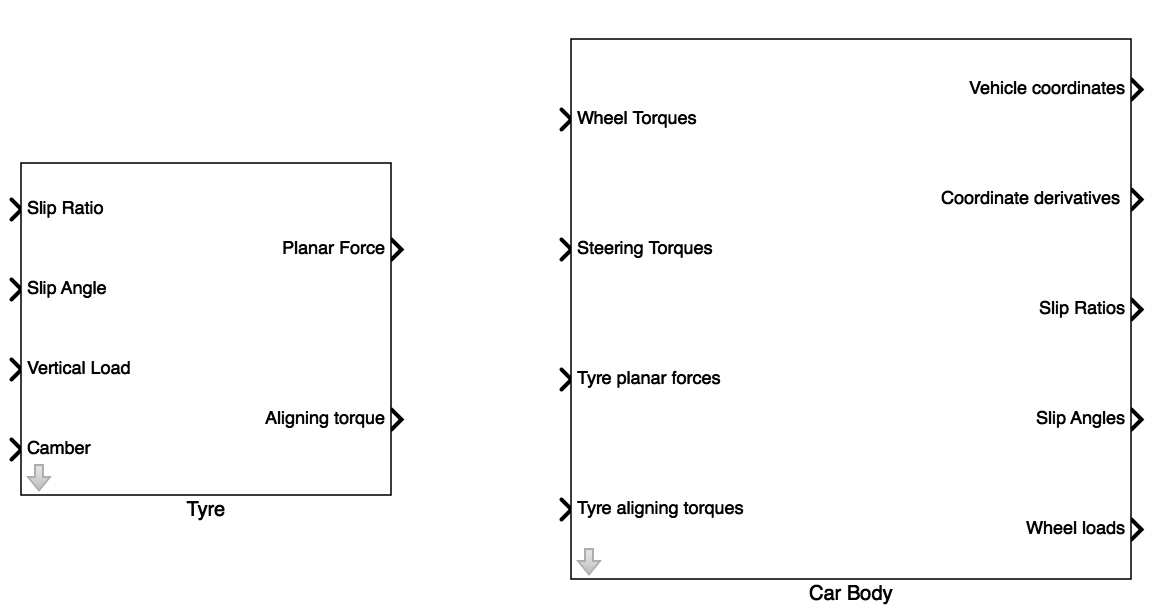
\includegraphics[scale=0.5]{images/bodyblockmask.png}
    \caption{Simulink blocks containing the tyre model and the 12DoF model.}
    \label{blocks}
\end{figure}

\section{Tyre block}

The Tyre model is implemented as a MATLAB function. The inputs are the slip ratio, the slip angle, the vertical force and the camber angle. The outputs are the horizontal force 2D vector $(F_x, F_y)$ and the aligning torque.
If all the tyres of the car are the same a single tyre block can be used to model all four wheels of the car, this is done by concantenating the inputs horizontally into a matrix. The forces corresponding to each tyre can then be extracted as columns of the outputs.
The outputs are computed by evaluating the Magic Formula equations described in \cite{pac2002}.
The coefficients representing the tyre for the simulations must be given in the Adams Car ".TIR" format. The format is human readable as a plaintext file, as described in \cite{pac2002}.
The tire model file must be located in the Matlab working directory. The name of the file can be entered in the "block mask" accessible by double clicking the block (Figure \ref{tyremask}).

\begin{figure}[ht]
    \centering
    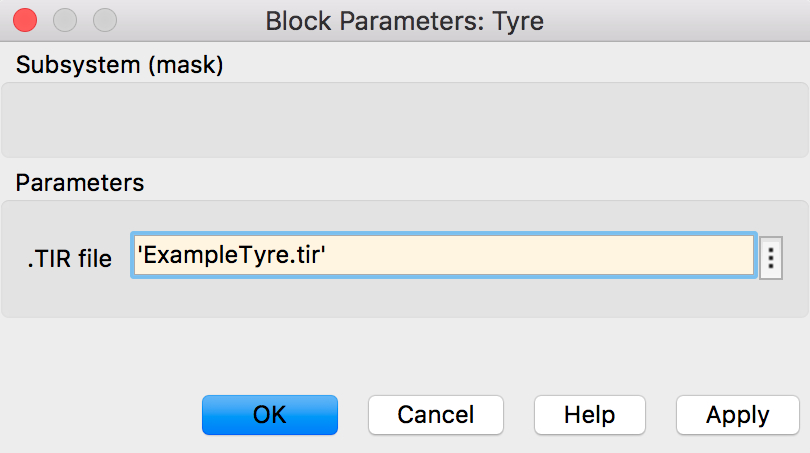
\includegraphics[scale=0.5]{images/tyremask.png}
    \caption{Simulink mask for the tyre block allows selection of the tyre model.}
    \label{tyremask}
\end{figure}

The parameters are loaded from the file into the tyre block workspace during the initialization phase by means of a script which takes advantage of the "loadTIR" function by Marco Furlan\cite{loadtir}.

Note that tyres are not always simmetrical. The model used in these simulations reflects this property and yields non-zero lateral force at zero slip angle. For this reason care should be taken when modelling tyres on opposite sides of the car. The ".TIR" files contain a field specifying for which side the empirical coefficients were fitted. To model tyres on the other side all inputs and outputs can be redefined in a simmetrical reference system. This simply means the slip angle and camber angle signs have to be changed before entering the tyre model and the lateral force and aligning moment signs have to be changed after they are output.

\section{Vehicle Body Block}
\label{sec:bodyblock}
The internal block diagram for the 12 DoF Model is shown in figure \ref{12diag}.
\begin{figure}[ht]
    \centering
    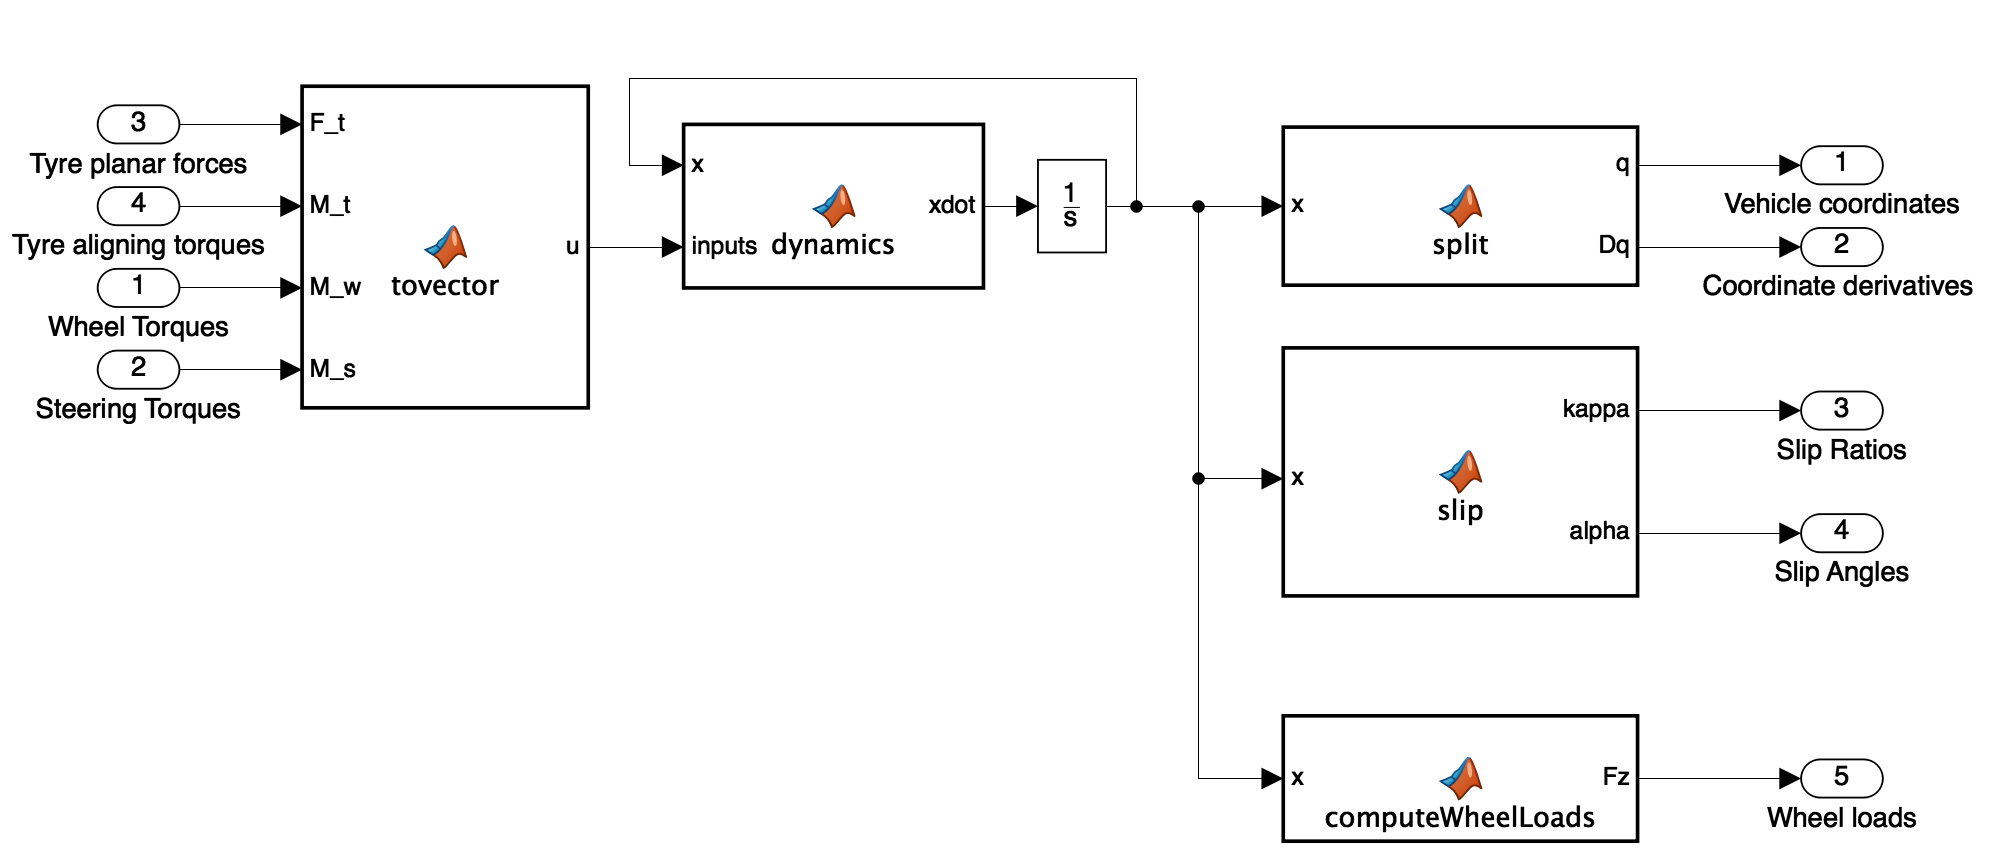
\includegraphics[width=\textwidth]{images/12dofinside.png}
    \caption{Simulink block diagram for the 12DoF model.}
    \label{12diag}
\end{figure}
The dynamics block employs the state space representation of the system to evaluate the state derivative $\dot x$ from the state and the inputs. $\dot x$ is then integrated completing it's feedback loop.
The "tovector" block simply assembles the incoming signals into the input vector for the dynamic system. The "split" block disassembles the state vector $x$ into the lagragian coordinates and their derivatives.
The "slip" block takes the vehicle coordinates as an input, calculates the contact point velocities and returns the slip angles and slip ratios.
The "computeWheelLoads" block evaluates the vertical wheel forces using the formulas in section \ref{sec:6dofout}.

\subsection{Parameters and initial state}
The initial state for the integrator and the vehicle body parameters are taken from text files. The text files are in the format shown in figures \ref{params} and \ref{init}.
The file names are entered in the block mask as seen in \ref{12mask}.

\begin{figure}[ht]
\begin{verbatim}
# car parameters file,  variable names must match those used in carmodel.m
# all units are metric
g          9.81       # gravity
t_f        1.2        # front track
t_r        1.2        # rear track
l_f        0.8        # Front axle to CG distance
l_r        0.8        # Rear axle to CG distance
q_f        0.09       # front roll center height
q_r        0.09       # rear roll center height
h_CG       0.3        # CG height
I_f        1          # Front Steering inertia
I_r        1          # Rear steering Inertia
k_f        35000      # front virtual spring stiffness
k_r        35000      # rear virtual spring stiffness
b_f        2000       # front virtual suspension damping
b_r        2000       # rear virtual suspension damping
m          300        # sprung mass (including driver)
m_u        50         # unsprung mass
Ixx        30         # Moment of inertia about longitudinal axis (sprung only)
Iyy        60         # Moment of inertia about lateral axis (sprung only)
Izz        50         # Moment of inertia about vertical axis (sprung only)
Ixz        0          # vertical-longitudinal inertia coupling
I_u        50         # unsprung mass rotational inertia about vertical axis
r_0        0.26       # wheel radius
I_w        0.3        # wheel rotational inertia
\end{verbatim}
\caption{Structure for the vehicle parameters file}
\label{params}
\end{figure}

\begin{figure}[ht]
\begin{verbatim}
# initial state file, variable names must match those used in carmodel.m
# all units are metric SI
y         0        # initial yaw
p         0        # initial pitch
r         0        # initial roll
x_CG      0        # initial CG coordinates
y_CG      0        # initial CG coordinates
z_CG     -0.3      # initial CG coordinates
delta_f   0        # initial front steer angle
delta_r   0        # initial rear steer angle
gamma_fr  0        # initial wheel angular position (FR)
gamma_fl  0        # initial wheel angular position (FL)
gamma_rr  0        # initial wheel angular position (RR)
gamma_rl  0        # initial wheel angular position (RL)
Dy        0        # initial yaw rate
Dp        0        # initial pitch rate
Dr        0        # initial roll rate
Dx_CG     1        # initial CG velocity wrt inertial frame
Dy_CG     0        # initial CG velocity wrt inertial frame
Dz_CG     0        # initial CG velocity wrt inertial frame
Ddelta_f  0        # initial front steering rate
Ddelta_r  0        # initial rear steering rate
Dgamma_fr 0        # initial wheel speed (FR)
Dgamma_fl 0        # initial wheel speed (FL)
Dgamma_rr 0        # initial wheel speed (RR)
Dgamma_rl 0        # initial wheel speed (RL)
\end{verbatim}
\caption{Structure for the initial vehicle state file}
\label{init}
\end{figure}

\begin{figure}[ht]
    \centering
    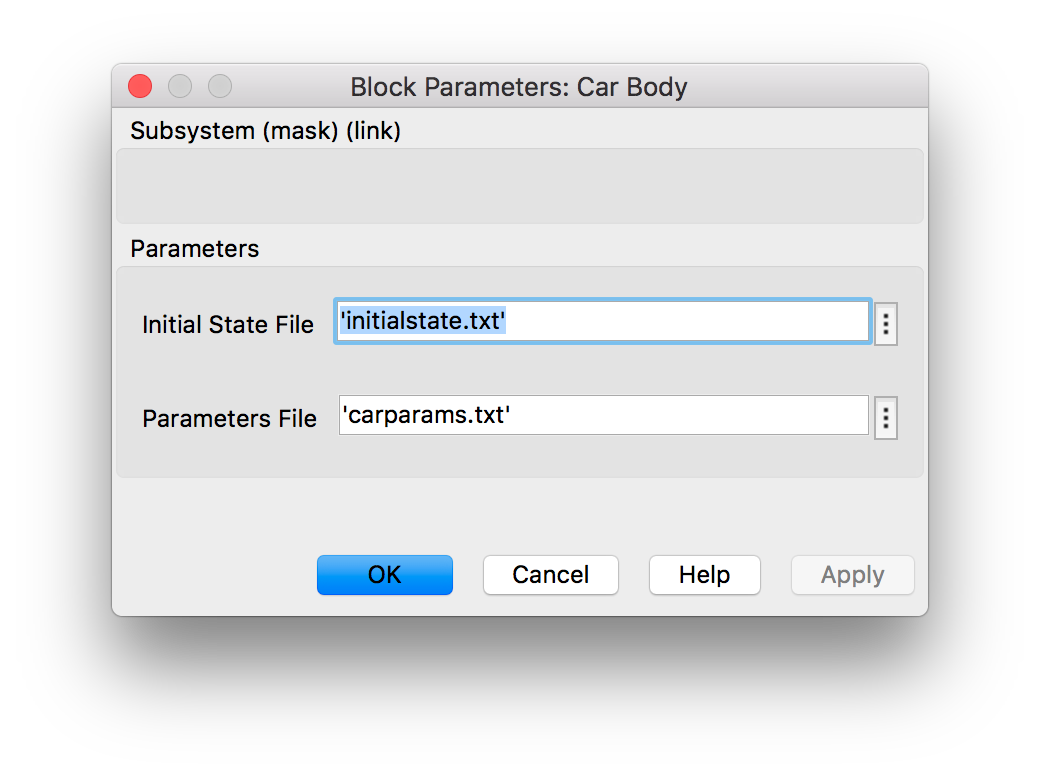
\includegraphics[width=\textwidth]{images/bodymask.png}
    \caption{Simulink block mask for the body dynamics Model.}
	\label{12mask}
\end{figure}

\section{Simulation diagram}
To obtain interesting data from a vehicle dynamics simulation the car model needs to receive a realistic input. Inputs for testing the discussed model were generated in different ways.

The first tests were done without the intervention of the tyre model. Constant forces or torques were directly applied to the model inputs to verify the expected behaviour.
After debugging the vehicle body model using this method the tyre model was connected, the resulting block diagram for the 12 DoF model is as shown in figure \ref{12doftest}.

\begin{sidewaysfigure}[ht]
    \centering
    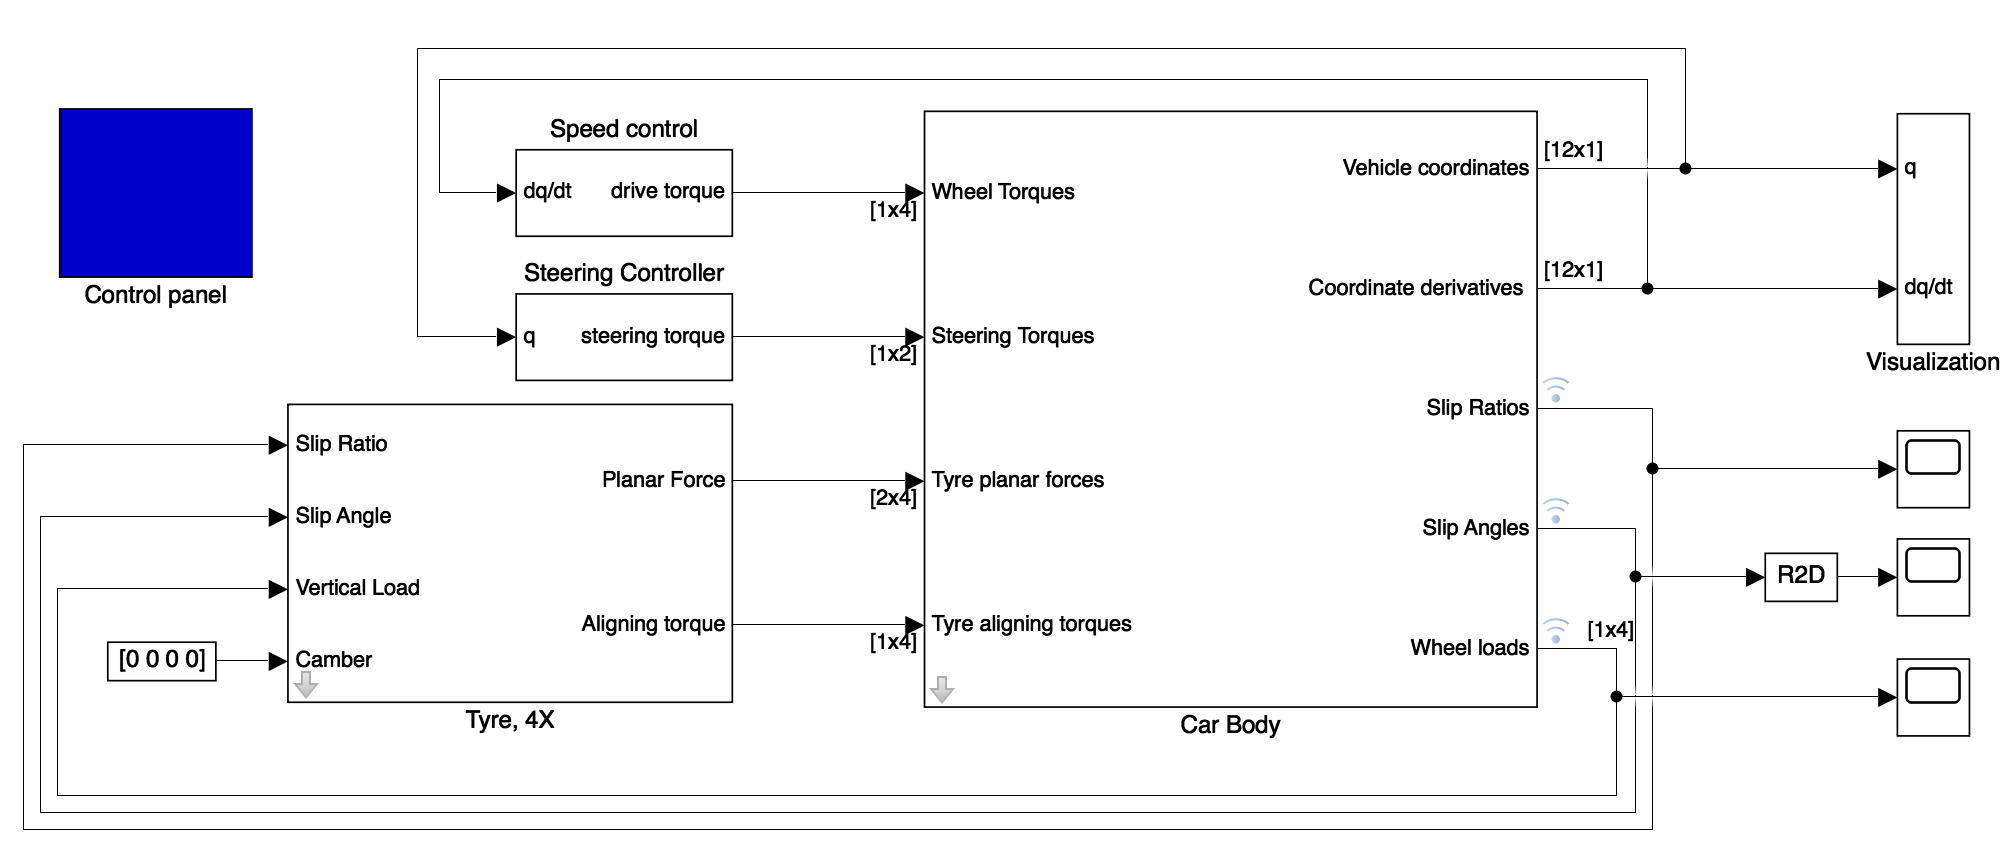
\includegraphics[width=\textwidth]{images/12doftest.png}
    \caption{Block diagram with steering and speed controllers for test simulations.}
    \label{12doftest}
\end{sidewaysfigure}

The Steering and Speed controllers may be implemented in various ways to obtain the desired test conditions.

\subsection{Skidpad test}
A skidpad test consists in driving the examined vehicle in a circle with constant radius and at constant speed. This kind of test is easy to reproduce experimentally and is thus useful in validation of vehicle dynamics models. 

Maintaining constant speed is done by using a PID controller whose output is the (equal) torque applied to the rear wheels.

Following a circular trajectory can be seen as holding a constant distance from the origin of the inertial reference system. This was accomplished by using two controllers.

The first PID controller acts in a servo loop to hold a target steering angle.

The second PID controller generates the target steering angle to hold the desired trajectory.
